% (c) 2017 Daniele Zambelli - daniele.zambelli@gmail.com
% 
% Tutti i grafici per il capitolo relativo alle funzioni_new
% 

\usetikzlibrary{shapes.gates.logic.US,trees,positioning,arrows}

% \newcommand{\grafiscatola}{% 
%   % Funzione rappresentata la funzione come scatola nera
%   \disegno[10]{
%      \node [draw, fill=blue!20, minimum size=3em, rounded corners] 
%             at (0, 0) (block 1) {add};
%      \draw [->] (-1, -0.5) node [left] {$o_1$} -- (block 1);
%      \draw [->] (-1, +0.5) node [left] {$o_2$} -- (block 1);
%      \draw[->] (block 1.east) -- (1, 0) node [right] {somma};
%         
%      \node [draw, fill=blue!20, minimum size=3em, rounded corners] 
%             at (0, 2) (block 2) {add};
%      \draw [->] (1, 1.5) node [right] {$o_1$} -- (block 2);
%      \draw [->] (1, +2.5) node [right] {$o_2$} -- (block 2);
%      \draw[->] (block 2.west) -- (-1, 2) node [left] {somma};
%   }
% }

\newcommand{\scatolasommasda}{% 
  \disegno[10]{
     \node [draw, fill=blue!20, minimum size=3em, rounded corners] 
            at (0, 0) (block 1) {add};
     \draw [->] (-1, +0.5) node [left] {$o_1$} -- (block 1);
     \draw [->] (-1, -0.5) node [left] {$o_2$} -- (block 1);
     \draw[->] (block 1.east) -- (1, 0) node [right] {somma};
  }
}

\newcommand{\scatolasommadsa}{% 
  \disegno[10]{
     \node [draw, fill=blue!20, minimum size=3em, rounded corners] 
            at (0, 2) (block 2) {add};
     \draw [->] (1, +2.5) node [right] {$o_1$} -- (block 2);
     \draw [->] (1, 1.5) node [right] {$o_1$} -- (block 2);
     \draw[->] (block 2.west) -- (-1, 2) node [left] {somma};
  }
}

\newcommand{\grafoscatolasd}[4]{% 
  % Funzione binaria rappresentata come scatola nera a sinistra
  % esempio di chiamata:
  % \grafoscatolasx{add}{o_1}{o_2}{somma}
  \def \nomef{#1}
  \def \opa{#2}
  \def \opb{#3}
  \def \risultato{#4}
  \disegno[10]{
     \node [draw, fill=blue!20, minimum size=3em, rounded corners] 
            at (0, 0) (block 1) {\nomef};
     \draw [->] (-1, +0.5) node [left] {$\opa$} -- (block 1);
     \draw [->] (-1, -0.5) node [left] {$\opb$} -- (block 1);
     \draw[->] (block 1.east) -- (1, 0) node [right] {$\risultato$};
  }
}

\newcommand{\grafoscatolads}[4]{% 
  % Funzione binaria rappresentata come scatola nera a destra
  % esempio di chiamata:
  % \grafoscatoladx{add}{7}{5}{12}
  \def \nomef{#1}
  \def \opa{#2}
  \def \opb{#3}
  \def \risultato{#4}
  \disegno[10]{
     \node [draw, fill=blue!20, minimum size=3em, rounded corners] 
            at (0, 2) (block 2) {\nomef};
     \draw [->] (1, +2.5) node [right] {$\opa$} -- (block 2);
     \draw [->] (1, 1.5) node [right] {$\opb$} -- (block 2);
     \draw[->] (block 2.west) -- (-1, 2) node [left] {$\risultato$};
  }
}

\begin{comment}
 You can define a new style that automates setting the start coordinate and 
drawing the arc:

\tikzset{
    partial ellipse/.style args={#1:#2:#3}{
        insert path={+ (#1:#3) arc (#1:#2:#3)}
    }
}

Then you can simply say

\draw[thick, red, -latex] (0,0) [partial ellipse=30:150:3cm and 2cm];


\begin{tikzpicture}
 
% Arc operation
\draw (2,0) arc
    [
        start angle=0,
        end angle=300,
        x radius=2cm,
        y radius =1cm
    ] ;
 
\end{tikzpicture}
 
 
 
\end{comment}


\newcommand{\grafoportad}[5][1]{% 
  % Funzione binaria rappresentata come porta logica
  % esempio di chiamata:
  % \grafoportad[3]{add}{o_1}{o_2}{somma}
  \def \dim{#1}
  \def \nomef{#2}
  \def \opa{#3}
  \def \opb{#4}
  \def \risultato{#5}
  \def \ddim{2*\dim}
  \disegno{
    \draw (0, 0) node {\nomef} (-\dim, +\dim) -- (-\dim, -\dim) 
      arc [start angle=-90, end angle=90, x radius=\ddim, y radius =\dim]
      -- cycle;
     \draw (-1.5*\dim, .5*\dim) node [left=-4pt] {$\boxed{\opa}$} -- 
       (-\dim, .5*\dim)
       (-1.5*\dim, -.5*\dim) node [left=-4pt] {$\boxed{\opb}$} -- 
       (-\dim, -.5*\dim)
       (+\dim, 0) -- (+1.5*\dim, 0) 
       node [right=-4pt] {$\boxed{\risultato}$};
  }
}

\newcommand{\grafoportas}[5][1]{% 
  % Funzione binaria rappresentata come porta logica
  % esempio di chiamata:
  % \grafoportas{add}{o_1}{o_2}{somma}
  \def \dim{#1}
  \def \nomef{#2}
  \def \opa{#3}
  \def \opb{#4}
  \def \risultato{#5}
  \def \ddim{2*\dim}
  \disegno{
    \draw (0, 0) node {\nomef} (+\dim, -\dim) -- (+\dim, +\dim) 
      arc [start angle=+90, end angle=270, x radius=\ddim, y radius =\dim]
      -- cycle;
     \draw (+1.5*\dim, .5*\dim) node [right=-4pt] {$\boxed{\opa}$} -- 
       (+\dim, .5*\dim)
       (+1.5*\dim, -.5*\dim) node [right=-4pt] {$\boxed{\opb}$} -- 
       (+\dim, -.5*\dim)
       (-\dim, 0) -- (-1.5*\dim, 0) 
       node [left=-4pt] {$\boxed{\risultato}$};
  }
}

\newcommand{\nodoesp}[7][]{% nodo di un'espressione numerica
  % IMPORTANTE: si aspetta che nel suo ambiente sia definita la variabile:
  % \ndim, ad esempio:
  % \def \ndim{.94}
  % esempio di chiamata:
  % \nodoesp{(-5, -1)}{(-4, -1)}{-4.5}{-3}{\times}{12}
  \def \rdim{#1}
  \def \popa{#2}
  \def \popb{#3}
  \def \xris{#4}
  \def \yris{#5}
  \def \nop{#6}
  \def \nris{#7}
  \def \ndim{1.0}
  \def \dimalf{\ndim/2}
  \def \ddim{\ndim/10}
  \def \xtopl{\xris-\dimalf}
  \def \xtopr{\xris+\dimalf}
  \def \ytop{\yris+2*\ndim}
  \def \ym{\yris+3*\dimalf}
  \draw \popa to [out=270, in=90] (\xris-3*\ddim, \ytop);
  \draw \popb to [out=270, in=90] (\xris+3*\ddim, \ytop);
  \draw (\xtopl, \ytop) -- (\xtopr, \ytop) -- (\xtopr, \ym) 
        arc (0:-180:\dimalf) -- cycle;
  \draw (\xris, \ym) node {\rdim$\nop$}
        (\xris, \yris) node[draw, above, rectangle,rounded corners=1pt] 
                           {\rdim$\nris$};
%         (\xris, \yris) node[draw, above, rectangle] {$\ris$};
  
}

\newcommand{\parentesi}[5]{
  \def \posx{#1}
  \def \posy{#2}
  \def \inter{#3}
  \def \pa{#4}
  \def \pb{#5}
  \draw (\posx-\inter, \posy) node [above=-2pt] {$\pa$}
        (\posx+\inter, \posy) node [above=-2pt] {$\pb$};
  
}

\newcommand{\opfun}[7]{
  \def \oa{#1}
  \def \op{#2}
  \def \ob{#3}
  \def \ris{#4}
  \def \pa{#5}
  \def \pr{#6}
  \def \pb{#7}
  \def \la{-0.3}
  \def \lb{-2.8}
%   \def \ndim{1.0}
%   \def \xa{\pa} \def \xb{\pr} \def \xc{\pb}
  \disegno{
    \draw (0, 0) node{$\oa ~\op~ \ob$};
    \nodoesp{(\pa, \la)}{(\pb, \la)}{\pr}{\lb}{\op}{\ris}
  }
}

\newcommand{\addline}{
 \begin{tikzpicture}[decoration={markings,mark=between positions 0.7 and .9 
step 30pt with {\arrow{stealth}}}]
  \begin{scope}[thick,font=\scriptsize]
   \draw[->] (0,0)  - -  (280pt,0) node[above]{$\N$};
    \foreach \c in {3,4,...,7}{%
     \draw[dotted, color=RedOrange,postaction={decorate}](\c,5pt)--(\c,5pt) 
arc (180:0:0.5 and 0.5);}
    \foreach \n in {0,1,2,...,9}{%	
     \draw (\n,-3pt) -- (\n,3pt)   node [below=5pt] {$\n$};}
  \end{scope}
 \end{tikzpicture}
}

\newcommand{\defpot}{
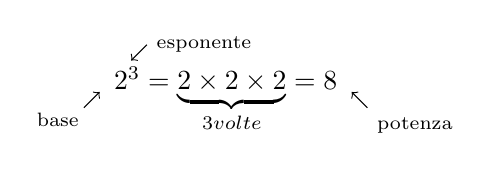
\begin{tikzpicture} 
  \node (esp) at (0,0) 
    {$2^3=\underbrace{2\times 2\times 2}_{3 \text{ volte}} = 8$};
\begin{scope}[font=\scriptsize]
  \draw[<-]  (-1.2,.5)--(-1,.7) node[right] {esponente};
  \draw[->]  (-1.8,-.1)--(-1.6,.1) node[below left=.2] {base};
  \draw[<-]  (1.6,.1)--(1.8,-.1) node[below right] {potenza };
\end{scope}
\end{tikzpicture}
}

\newcommand{\potfun}{
  \def \oa{2}
  \def \op{\uparrow}
  \def \ob{3}
  \def \ris{8}
  \def \la{-0.3}
  \def \lb{-2.8}
%   \def \ndim{1.0}
  \def \xa{-.2} \def \xb{0} \def \xc{+.2}
  \disegno{
    \draw (0, 0) node{$\oa^\ob$};
    \nodoesp{(\xa, \la)}{(\xc, -.1)}{\xb}{\lb}{\op}{\ris}
  }
}

\newcommand{\sotline}{
 \begin{tikzpicture}[decoration={markings,mark=between positions .3 and .5 
step 30pt with {\arrowreversed{stealth}}}]
  \begin{scope}[thick,font=\scriptsize]
   \draw[->] (0,0)  - -  (280pt,0) node[above]{$\N$};
    \foreach \c in {2,3,...,6}{%
     \draw[dotted, color=CornflowerBlue, postaction={decorate}]
       (\c,5pt) -- (\c,5pt) arc (180:0:0.5 and 0.5);}
    \foreach \n in {0,1,2,...,9}{%	
     \draw (\n,-3pt) -- (\n,3pt)   node [below=5pt] {$\n$};}
  \end{scope}
 \end{tikzpicture}
}

% \newcommand{\sotfun}{
%   \opfun{7}{-}{5}{2}
%   \def \oa{7}
%   \def \op{-}
%   \def \ob{5}
%   \def \ris{2}
%   \def \la{-0.3}
%   \def \lb{-2.8}
% %   \def \ndim{1.0}
%   \def \xa{-.8} \def \xb{0} \def \xc{+.8}
%   \disegno{
%     \draw (0, 0) node{\(\oa ~\op~ \ob\)};
%     \nodoesp{(\xa, \la)}{(\xc, \la)}{\xb}{\lb}{\op}{\ris}
%   }
% }

\newcommand{\assocsinistra}{
  \def \la{-0.3}
  \def \lb{-2.8}
  \def \lc{-5.3}
%   \def \ndim{1.0}
  \def \xa{-1.6} \def \xb{-0.8} \def \xc{-.1} \def \xd{+.8} \def \xe{+1.6}
  \disegno{
    \draw (0, 0) node{$7 ~+~ 5 ~\times~ 2$};
    \nodoesp{(\xa, \la)}{(\xc, \la)}{\xb}{\lb}{+}{12}
    \nodoesp{(\xb, \lb)}{(\xe, \la)}{\xd}{\lc}{\times}{24}
  }
}

\newcommand{\precedenzaalg}{
  \def \la{-0.3}
  \def \lb{-2.8}
  \def \lc{-5.3}
  \def \ndim{1.0}
  \def \xa{-1.6} \def \xb{-0.8} \def \xc{-.1} \def \xd{+.8} \def \xe{+1.6}
  \disegno{
    \draw (0, 0) node{$7 ~+~ 5 ~\times~ 2$};
    \nodoesp{(\xc, \la)}{(\xe, \la)}{\xd}{\lb}{\times}{10}
    \nodoesp{(\xa, \la)}{(\xd, \lb)}{\xb}{\lc}{+}{17}
  }
}

\newcommand{\espalberoav}{
  \def \la{-0.3}
  \def \lb{-2.8}
  \def \lc{-5.3}
  \def \ld{-7.0}
  \def \le{-8.7}
%   \def \ndim{1.0}
  \def \xa{-4.5} \def \xb{-3.5} 
  \def \xc{-2.55} \def \xd{-2.35} \def \xe{-2.15} 
  \def \xf{-1.45} 
  \def \xg{-0.1} \def \xh{+0.63} \def \xi{+1.25} 
  \def \xj{+2.37} \def \xk{+3.3} 
  \disegno{
%     \foreach \x/\l in {\xa/a, \xb/b, \xc/c, \xd/d, \xe/e, 
%                        \xf/f, \xg/g, \xh/h, \xi/i, \xj/j, 
%                        \xk/k %, \xl/l, \xm/m, \xn/n, \xo/o, 
% %                        \xp/p, \xq/q, \xr/r, \xs/s, \xt/t,
% %                        \xu/u, \xv/v, \xw/w, \xx/x, \xy/y, 
% %                        \xz/z, \xaa/a
%                        }{
%       \draw (\x, \la) circle(1pt) node [below] {\l};
%     }
    \draw (0, 0) node{
    $49 ~-~ [2^4 ~\times~ (14 ~:~ 7) ~+~ 10]~=$};
    \nodoesp{(\xc, \la)}{(\xe, 0)}{\xd}{\lb}{\uparrow}{\phantom{16}}
    \nodoesp{(\xg, \la)}{(\xi, \la)}{\xh}{\lb}{\div}{\phantom{2}}
    \parentesi{\xh}{\lb}{.8}{(}{)}
    \nodoesp{(\xd, \lb)}{(\xh, \lb)}{\xf}{\lc}{\times}{\phantom{32}}
    \nodoesp{(\xf, \lc)}{(\xk, \la)}{\xj}{\ld}{+}{\phantom{42}}
    \parentesi{\xj}{\ld}{1}{[}{]}
    \nodoesp{(\xa, \la)}{(\xj, \ld)}{\xb}{\le}{-}{\phantom{7}}
    \draw (\xb, \le) 
      node[draw, above, rectangle,rounded corners=1pt, very thick] 
          {\phantom{$7$}};
  }
}

\newcommand{\espalberoa}{
  \def \la{-0.3}
  \def \lb{-2.8}
  \def \lc{-5.3}
  \def \ld{-7.0}
  \def \le{-8.7}
%   \def \ndim{1.0}
  \def \xa{-4.5} \def \xb{-3.5} 
  \def \xc{-2.55} \def \xd{-2.35} \def \xe{-2.15} 
  \def \xf{-1.45} 
  \def \xg{-0.1} \def \xh{+0.63} \def \xi{+1.25} 
  \def \xj{+2.37} \def \xk{+3.3} 
  \disegno{
%     \foreach \x/\l in {\xa/a, \xb/b, \xc/c, \xd/d, \xe/e, 
%                        \xf/f, \xg/g, \xh/h, \xi/i, \xj/j, 
%                        \xk/k %, \xl/l, \xm/m, \xn/n, \xo/o, 
% %                        \xp/p, \xq/q, \xr/r, \xs/s, \xt/t,
% %                        \xu/u, \xv/v, \xw/w, \xx/x, \xy/y, 
% %                        \xz/z, \xaa/a
%                        }{
%       \draw (\x, \la) circle(1pt) node [below] {\l};
%     }
    \draw (0, 0) node{
    $49 ~-~ [2^4 ~\times~ (14 ~:~ 7) ~+~ 10]~=$};
    \nodoesp{(\xc, \la)}{(\xe, 0)}{\xd}{\lb}{\uparrow}{16}
    \nodoesp{(\xg, \la)}{(\xi, \la)}{\xh}{\lb}{\div}{2}
    \parentesi{\xh}{\lb}{.8}{(}{)}
    \nodoesp{(\xd, \lb)}{(\xh, \lb)}{\xf}{\lc}{\times}{32}
    \nodoesp{(\xf, \lc)}{(\xk, \la)}{\xj}{\ld}{+}{42}
    \parentesi{\xj}{\ld}{1}{[}{]}
    \nodoesp{(\xa, \la)}{(\xj, \ld)}{\xb}{\le}{-}{7}
    \draw (\xb, \le) 
      node[draw, above, rectangle,rounded corners=1pt, very thick] 
          {$7$};
  }
}

\newcommand{\espalberob}{
  \def \la{-0.3}
  \def \lb{-2.8}
  \def \lc{-5.3}
  \def \ld{-7.8}
  \def \le{-10.3}
  \def \lf{-11.5}
%   \def \ndim{1.0}
  \def \xa{-6.9} \def \xb{-6} \def \xc{-5} 
  \def \xd{-4.3} \def \xe{-3.1} \def \xf{-2.75} \def \xg{-2.4} 
  \def \xh{-1.8} \def \xi{-0.7} \def \xj{0.27} 
  \def \xk{+1.4} \def \xl{+1.8} \def \xm{+2.15} \def \xn{+3.15} 
  \def \xo{+4.15} \def \xp{+5.2} \def \xq{+6.} 
  \disegno{
%     \foreach \x/\l in {\xa/a, \xb/b, \xc/c, 
%                        \xd/d, 
%                        \xe/e, \xf/f, \xg/g, 
%                        \xh/h, 
%                        \xi/i, \xj/j, 
%                        \xk/k , \xl/l, \xm/m, \xn/n, \xo/o, 
%                        \xp/p, \xq/q%, \xr/r, \xs/s, \xt/t,
% %                        \xu/u, \xv/v, \xw/w, \xx/x, \xy/y, 
% %                        \xz/z, \xaa/a, \xaa/a, \xaa/a, \xaa/a, 
% %                        \xaa/a
%                        }{
%       \draw (\x, \la) circle(1pt) node [below] {\l};
%     }
    \draw (0, 0) node{
    $8^9 ~\times~ 8^5 ~:~ (8^3)^4 ~:~ 
    [4^{12} ~:~ (4^2)^5] ~+~ 27^2 ~:~ 9^2 ~=$};
    \nodoesp[\footnotesize]{(\xa, \la)}{(\xc, \la)}{\xb}{\lb}{p1}{8^{14}}
    \nodoesp[\footnotesize]{(\xe, \la)}{(\xg, 0)}{\xf}{\lb}{p3}{8^{12}}
    \nodoesp[\footnotesize]{(\xk, \la)}{(\xm, 0)}{\xl}{\lb}{p3}{4^{10}}
    \nodoesp[\footnotesize]{(\xo, \la)}{(\xq, \la)}{\xp}{\lb}{p5}{3^{2}}
    \nodoesp[\footnotesize]{(\xb, \lb)}{(\xf, \lb)}{\xd}{\lc}{p2}{8^{2}}
    \nodoesp[\footnotesize]{(\xi, \la)}{(\xl, \lb)}{\xj}{\lc}{p2}{4^{2}}
    \nodoesp{(\xp-.2, \lb+.2)}{(\xp+.2, \lb+.4)}{\xp}{\lc}{\uparrow}{9}
    \nodoesp{(\xd-.2, \lc+.2)}{(\xd+.2, \lc+.4)}{\xd}{\ld}{\uparrow}{64}
    \nodoesp{(\xj-.2, \lc+.2)}{(\xj+.2, \lc+.4)}{\xj}{\ld}{\uparrow}{16}
    \parentesi{\xj}{\ld}{1}{[}{]}
    \nodoesp{(\xd, \ld)}{(\xj, \ld)}{\xh}{\le}{\div}{4}
    \nodoesp{(\xh, \le)}{(\xp, \lc)}{\xn}{\lf}{+}{13}
    \draw (\xn, \lf) 
      node[draw, above, rectangle,rounded corners=1pt, very thick] {$13$};
  }
}

\newcommand{\espalberoc}{
  \def \la{-0.3}
  \def \lb{-2.8}
  \def \lc{-5.3}
  \def \ld{-7.5}
  \def \le{-8.7}
  \def \xa{-4.5} \def \xb{-4.3} \def \xc{-4.1} 
  \def \xd{-3.4} 
  \def \xe{-2.3} \def \xf{-2.1} \def \xg{-1.9} 
  \def \xh{-1.2} \def \xi{-0.4} \def \xj{+0.4} 
  \def \xk{+1.35} \def \xl{+1.65} \def \xm{+1.85} 
  \def \xn{+2.45} 
  \def \xo{+3.05} \def \xp{+3.25} \def \xq{+3.45} 
  \disegno{
%     \foreach \x/\l in {\xa/a, \xb/b, \xc/c, \xd/d, \xe/e, 
%                        \xf/f, \xg/g, \xh/h, \xi/i, \xj/j, 
%                        \xk/k, \xl/l, \xm/m, \xn/n, \xo/o, 
%                        \xp/p, \xq/q%, \xr/r, \xs/s, \xt/t,
% %                        \xu/u, \xv/v, \xw/w, \xx/x, \xy/y, 
% %                        \xz/z, \xaa/a
%                        }{
%       \draw (\x, \la) circle(1pt) node [below] {\l};
%     }
    \draw (0, 0) node{
    $[3^3 ~-~ \tonda{5^2 ~\times~ 2 ~-~ 10^2 ~:~ 2^2} ~=$};
    \nodoesp{(\xa, \la)}{(\xc, 0)}{\xb}{\lb}{\uparrow}{27}
    \nodoesp{(\xe, \la)}{(\xg, 0)}{\xf}{\lb}{\uparrow}{25}
    \nodoesp{(\xk, \la)}{(\xm, 0)}{\xl}{\lb}{\uparrow}{100}
    \nodoesp{(\xo, \la)}{(\xq, 0)}{\xp}{\lb}{\uparrow}{4}
    \nodoesp{(\xf, \lb)}{(\xi, \la)}{\xh}{\lc}{\times}{50}
    \nodoesp{(\xl, \lb)}{(\xp, \lb)}{\xn}{\lc}{\div}{25}
    \nodoesp{(\xh, \lc)}{(\xn, \lc)}{\xj}{\ld}{-}{25}
    \parentesi{\xj}{\ld}{1}{(}{)}
    \nodoesp{(\xb, \lb)}{(\xj, \ld)}{\xd}{\le}{-}{2}
    \draw (\xd, \le) 
      node[draw, above, rectangle,rounded corners=1pt, very thick] 
          {$2$};
  }
}

% \phantom{}
% \mathcolor{blue}{b}
% \textcolor{blue}{b}

\newcommand{\espbucoabase}{
  \def \la{-0.3}
  \def \lb{-2.8}
  \def \lc{-5.3}
  \def \ld{-7.3}
  \def \le{-8.7}
  \def \lf{-10.5}
%   \def \ndim{1.0}
  \def \xa{-6.9} \def \xb{-6.15} 
  \def \xc{-5.4} \def \xd{-4.57} \def \xe{-3.6} 
  \def \xf{-2.8} \def \xg{-2.15} \def \xh{-1.35} 
  \def \xi{-0.1} \def \xj{+0.85} \def \xk{+1.65} 
  \def \xl{+1.85} \def \xm{+2.05} \def \xn{+3.2} 
  \def \xo{+3.95} \def \xp{+4.82} \def \xq{+5.45} 
%     \foreach \x/\l in {\xa/a, \xb/b, \xc/c, \xd/d, \xe/e, 
%                        \xf/f, \xg/g, \xh/h, \xi/i, \xj/j, 
%                        \xk/k, \xl/l, \xm/m, \xn/n, \xo/o, 
%                        \xp/p, \xq/q%, \xr/r, \xs/s, \xt/t,
% %                        \xu/u, \xv/v, \xw/w, \xx/x, \xy/y, 
% %                        \xz/z, \xaa/a
%                        }{
%       \draw (\x, \la) circle(1pt) node [below] {\l};
%     }
    \draw (0, 0) node{
    $[4 ~\times~ 5 ~+~ 16 ~:~ 2 ~-~ (13 ~-~ 2^{\dots}) ~\times~ 2] ~:~ 
      2 ~=~ 9$};
    \nodoesp{(\xa, \la)}{(\xc, \la)}{\xb}{\lb}{\times}{20}
    \nodoesp{(\xe, \la)}{(\xg, \la)}{\xf}{\lb}{\div}{8}
    \nodoesp{(\xk, \la)}{(\xm, 0)}{\xl}{\lb}{\uparrow}{\phantom{8}}
    \nodoesp{(\xb, \lb)}{(\xf, \lb)}{\xd}{\lc}{+}{28}
    \nodoesp{(\xi, \la)}{(\xl, \lb)}{\xj}{\lc}{-}{\phantom{5}}
    \parentesi{\xj}{\lc}{.8}{(}{)}
    \nodoesp{(\xj, \lc)}{(\xo, \la)}{\xn}{\ld}{\times}{\phantom{10}}
    \nodoesp{(\xd, \lc)}{(\xn, \ld)}{\xh}{\le}{-}{\phantom{18}}
    \parentesi{\xh}{\le}{1}{[}{]}
    \nodoesp{(\xh, \le)}{(\xq, \la)}{\xp}{\lf}{\div}{\phantom{9}}
    \draw (\xp, \lf) 
      node[draw, above, rectangle,rounded corners=1pt, very thick] 
          {$\textcolor{blue}{9}$};
}

\newcommand{\espbucoaa}{
  \disegno{
    \espbucoabase
    \draw (\xh, \le) node [above]
      {\footnotesize$~\textcolor{blue}{\bigstar}~$};
  }
}

\newcommand{\espbucoab}{
  \disegno{
    \espbucoabase
    \draw (\xh, \le) node [above]{$\textcolor{blue}{18}$};
    \draw (\xn, \ld) node [above]
      {\footnotesize$~\textcolor{blue}{\bigstar}~$};
  }
}

\newcommand{\espbucoac}{
  \disegno{
    \espbucoabase
    \draw (\xh, \le) node [above]{$\textcolor{blue}{18}$};
    \draw (\xn, \ld) node [above]{$\textcolor{blue}{10}$};
    \draw (\xj, \lc) node [above]{$\textcolor{blue}{5}$};
    \draw (\xl, \lb) node [above]{$\textcolor{blue}{8}$};
    \draw (\xm, 0.3) node {\footnotesize$\textcolor{blue}{3}$};
  }
}

\newcommand{\espbucob}{
  \def \la{-0.3}
  \def \lb{-2.8}
  \def \lc{-5.3}
  \def \ld{-7.8}
  \def \le{-10.3}
  \def \lf{-12.3}
%   \def \ndim{1.0}
  \def \xa{-7.6} \def \xb{-7.1} \def \xc{-6.8} 
  \def \xd{-6.1} \def \xe{-5.3} \def \xf{-4.35} 
  \def \xg{-3.4} \def \xh{-3.0} \def \xi{-2.65} \def \xj{-1.9} 
  \def \xk{-1.1} \def \xl{+0.0} \def \xm{+0.7} \def \xn{+1.55} 
  \def \xo{+2.75} \def \xp{+3.75} \def \xq{+4.5} 
  \def \xr{+5.33} \def \xs{+6.1} 
  \disegno{
%     \foreach \x/\l in {\xa/a, \xb/b, \xc/c, 
%                        \xd/d, 
%                        \xe/e, \xf/f, \xg/g, 
%                        \xh/h, 
%                        \xi/i, \xj/j, 
%                        \xk/k , \xl/l, \xm/m, \xn/n, \xo/o, 
%                        \xp/p, \xq/q, \xr/r, \xs/s%, \xt/t,
% %                        \xu/u, \xv/v, \xw/w, \xx/x, \xy/y, 
% %                        \xz/z, \xaa/a, \xaa/a, \xaa/a, \xaa/a, 
% %                        \xaa/a
%                        }{
%       \draw (\x, \la) circle(1pt) node [below] {\l};
%     }
    \draw (0, 0) node{
    $(3^4)^3 ~\times~ 3^{\dots} : (3^3)^5 ~-~ 2^3 ~\times~ 2 
     ~\times~ (20 ~-~ 3 ~\times~ 5) ~=~ 1$};
    \nodoesp[\footnotesize]{(\xa, \la)}{(\xc, 0)}{\xb}{\lb}{p3}{3^{12}}
    \nodoesp[\footnotesize]{(\xg, \la)}{(\xi, 0)}{\xh}{\lb}{p3}{3^{15}}
    \nodoesp[\footnotesize]{(\xk, \la)}{(\xm, \la)}{\xl}{\lb}{p2}{8^{2}}
    \nodoesp{(\xq, \la)}{(\xs, \la)}{\xr}{\lb}{\times}{15}
    \nodoesp[\footnotesize]{(\xb, \lb)}{(\xe, \la)}{\xd}{\lc}{p1}
      {\phantom{8^{14}}}
    \nodoesp{(\xl-.2, \lb+.2)}{(\xl+.2, \lb+.4)}{\xl}{\lc}{\uparrow}{16}
    \nodoesp{(\xo, \la)}{(\xr, \lb)}{\xp}{\lc}{-}{5}
    \parentesi{\xp}{\lc}{.8}{(}{)}
    \nodoesp[\footnotesize]{(\xd, \lc)}{(\xh, \lb)}{\xf}{\ld}{p2}
      {\phantom{8^{14}}}
    \nodoesp[\footnotesize]{(\xf-.2, \ld+.2)}{(\xf+.2, \ld+.4)}{\xf}{\le}
      {\uparrow}{~\textcolor{blue}{\bigstar}}
    \nodoesp{(\xl, \lc)}{(\xp, \lc)}{\xn}{\ld}{\times}{80}
    \nodoesp{(\xf, \le)}{(\xn, \ld)}{\xj}{\lf}{-}{\phantom{1}}
%     \nodoesp[\footnotesize]{(\xe, \la)}{(\xg, 0)}{\xf}{\lb}{p3}{8^{12}}
%     \nodoesp[\footnotesize]{(\xk, \la)}{(\xm, 0)}{\xl}{\lb}{p3}{4^{10}}
%     \nodoesp[\footnotesize]{(\xo, \la)}{(\xq, \la)}{\xp}{\lb}{p5}{3^{2}}
%     \nodoesp[\footnotesize]{(\xi, \la)}{(\xl, \lb)}{\xj}{\lc}{p2}{4^{2}}
%     \nodoesp{(\xp-.2, \lb+.2)}{(\xp+.2, \lb+.4)}{\xp}{\lc}{\uparrow}{9}
%     \nodoesp{(\xd-.2, \lc+.2)}{(\xd+.2, \lc+.4)}{\xd}{\ld}{\uparrow}{64}
%     \nodoesp{(\xj-.2, \lc+.2)}{(\xj+.2, \lc+.4)}{\xj}{\ld}{\uparrow}{16}
%     \nodoesp{(\xd, \ld)}{(\xj, \ld)}{\xh}{\le}{\div}{4}
%     \nodoesp{(\xh, \le)}{(\xp, \lc)}{\xn}{\lf}{+}{13}
    \draw (\xj, \lf) 
      node[draw, above, rectangle,rounded corners=1pt, very thick] 
          {$\textcolor{blue}{1}$};
  }
}

% \newcommand{\espressionealberodia}{
%   \def \la{-0.3}
%   \def \lb{-2.8}
%   \def \lc{-5.3}
%   \def \ld{-7.8}
%   \def \le{-10.3}
%   \def \lf{-12.8}
%   \def \lg{-14.2}
%   \def \ndim{1.0}
%   \def \xa{-10.55} \def \xb{-9.62} 
%   \def \xc{-8.7} \def \xd{-7.85} \def \xe{-7.0} 
%   \def \xf{-6.05} 
%   \def \xg{-4.8} \def \xh{-3.9} \def \xi{-3.0} 
%   \def \xj{-2.05} 
%   \def \xk{-1.2} \def \xl{-1.0} \def \xm{-0.8} 
%   \def \xn{+0.1} 
%   \def \xo{+0.95} \def \xp{+1.9} \def \xq{2.7} 
%   \def \xr{+3.95} 
%   \def \xs{5.1} \def \xt{5.3} \def \xu{5.5} 
%   \def \xv{6.4} 
%   \def \xw{7.25} \def \xx{7.45} \def \xy{7.65} 
%   \def \xz{8.8} \def \xaa{9.7} 
%   \disegno{
% %     \foreach \x/\l in {\xa/a, \xb/b, \xc/c, \xd/d, \xe/e, 
% %                        \xf/f, \xg/g, \xh/h, \xi/i, \xj/j, 
% %                        \xk/k, \xl/l, \xm/m, \xn/n, \xo/o, 
% %                        \xp/p, \xq/q, \xr/r, \xs/s, \xt/t,
% %                        \xu/u, \xv/v, \xw/w, \xx/x, \xy/y, 
% %                        \xz/z, \xaa/a}{
% %       \draw (\x, \la) circle(1pt) node [below] {\l};
% %     }
%     \draw (0, 0) node{
%     $2 ~+~ 6 ~\times~ 2 ~\div 
%     \left[ \left(4 ~-~ 2 \right) \times~ 3^{2} ~-~ 3 ~\times~ 5 \right] ~+~
%     \left( 5^{2} ~+~ 2^{3} \right) ~\div~ 3 =$};
%     \nodoesp{(\xc, \la)}{(\xe, \la)}{\xd}{\lb}{\times}{12}
%     \nodoesp{(\xg, \la)}{(\xi, \la)}{\xh}{\lb}{-}{2}
%     \parentesi{\xh}{\lb}{.8}{(}{)}
%     \nodoesp{(\xk, \la)}{(\xm, +0.0)}{\xl}{\lb}{\uparrow}{9}
%     \nodoesp{(\xo, \la)}{(\xq, \la)}{\xp}{\lb}{\times}{15}
%     \nodoesp{(\xs, \la)}{(\xu, +0.0)}{\xt}{\lb}{\uparrow}{25}
%     \nodoesp{(\xw, \la)}{(\xy, +0.0)}{\xx}{\lb}{\uparrow}{8}
%     \nodoesp{(\xh, \lb)}{(\xl, \lb)}{\xj}{\lc}{\times}{18}
%     \nodoesp{(\xt, \lb)}{(\xx, \lb)}{\xv}{\lc}{+}{33}
%     \parentesi{\xv}{\lc}{1}{(}{)}
%     \nodoesp{(\xj, \lc)}{(\xp, \lb)}{\xn}{\ld}{-}{3}
%     \parentesi{\xn}{\ld}{.8}{[}{]}
%     \nodoesp{(\xv, \lc)}{(\xaa, \la)}{\xz}{\ld}{\div}{11}
%     \nodoesp{(\xd, \lb)}{(\xn, \ld)}{\xf}{\le}{\div}{4}
%     \nodoesp{(\xa, \la)}{(\xf, \le)}{\xb}{\lf}{+}{6}
%     \nodoesp{(\xb, \lf)}{(\xz, \ld)}{\xr}{\lg}{+}{17}
%     \draw (\xr, \lg) 
%       node[draw, above, rectangle,rounded corners=1pt, very thick] 
%           {$\ris$};
%   }
% }

%\newcommand{\grafoporta}{% 
%  % Funzione rappresentata come porta logica
  
% \begin{circuitikz}[rotate=-90]
% \draw (0,3) node[american and port] (A) {P1};
% \begin{scope}
% \ctikzset{tripoles/american or port/height=1.6}
% \draw (A.out) -- ++(0.5,0)
% node[american or port,
% number inputs=5,
% anchor=in 1] (B) {P2};
% \end{scope}
% \draw (0,1.5) node[american or port] (C) {P3};
% \draw (C.out) |- (B.in 2);
% \end{circuitikz}
 
%  \disegno[10]{
%    \draw (6,0) node[nand2ni,anchor=tip,draw] (n4) {}
%      (n4.z) -- +(0mm,-5mm)
%      (n4.b) |- ++(10mm,2mm) -- ++(0mm,2mm)
%      node[and2in,anchor=z,draw,fill=gray] (n3) {}
%      (n4.a) |- ++(-10mm,2mm) -- ++(0mm,2mm)
%      node[or3nni,anchor=tip,draw] (n2) {}
%      (n3.b) -- +(0mm,5mm) node[above] {$i_5$}
%      (n3.a) |- ++(-5mm,2mm)
%      coordinate (p) -- +(0mm,5mm) node[above] {$i_4$}
%      (n2.c) |- (p)
%      (n2.b) |- ++(6mm,12mm) -- +(0mm,5mm) node[above] {$i_3$}
%      (n2.a) -- +(0mm,8mm)
%      node[and2,anchor=tip,draw] (n1) {}
%      (n1.b) -- +(0mm,5mm) node[above] {$i_2$}
%      (n1.a) -- +(0mm,5mm) node[above] {$i_1$};
%  }
%}
